\documentclass[a4paper,14pt]{article} % 14й шрифт
\usepackage{extsizes}
\usepackage{cmap} % для кодировки шрифтов в pdf
\usepackage[T2A]{fontenc}
\usepackage[utf8]{inputenc}
\usepackage[russian]{babel}
\usepackage{amssymb,amsfonts,amsmath,amsthm} % математические дополнения от АМС
\usepackage[left=20mm, top=15mm, right=15mm, bottom=15mm, nohead, footskip=10mm]{geometry} % настройки полей документа
\usepackage{graphicx}
\usepackage{float}
\usepackage{textcomp}
\usepackage{subcaption}
\usepackage{amsthm}% настройки полей документа

\renewcommand{\rmdefault}{ftm} % Times New Roman
\frenchspacing

\usepackage{tikz}
\usetikzlibrary{positioning}
\usetikzlibrary{circuits}
\usetikzlibrary{circuits.ee}
\usetikzlibrary{circuits.ee.IEC}
\usetikzlibrary{circuits.logic.IEC}

\newtheorem{definition}{Определение}
\newtheorem{theorem}{Теорема}
 
\begin{document} % начало документа

 
% НАЧАЛО ТИТУЛЬНОГО ЛИСТА
\begin{center}
\hfill \break
\normalsize{Санкт-Петербургский государственный университет}\\ 
\hfill \break
\normalsize{Математико-механический факультет}\\
\normalsize{\textbf{Кафедра прикладной кибернетики}}\\
\hfill \break
\hfill \break 
\hfill \break
\hfill \break
\hfill\break
\hfill \break
\normalsize{Миронов Алексей Владиславович}\\
\hfill \break
\large{Оценка области захвата для систем ФАПЧ 3 порядка}\\
\hfill \break
\small{Выпускная квалификационная работа}\\
\hfill \break
\hfill \break
\hfill \break
\hfill \break
\hfill \break
\hfill \break
\end{center}
 
\hfill \break
\hfill \break
\hfill \break
 
 \small{
\begin{flushright}
Научный руководитель:\\
д.ф.-м. н., профессор Юлдашев~Р.\:В.
\break \break
\break \break
Рецензент:\\
Благов~М.\:В.
\end{flushright}
}
\hfill \break
\hfill \break
\hfill \break
\hfill \break
\hfill \break
\hfill \break
\hfill \break
\hfill \break
\hfill \break
\hfill \break
\begin{center} Санкт-Петербург \\
2020 \end{center}
\thispagestyle{empty} % выключаем отображение номера для этой страницы
% КОНЕЦ ТИТУЛЬНОГО ЛИСТА

% BEGIN ТOF TITLE PAGE
\begin{center}
\hfill \break
\normalsize{Saint Petersburg State University}\\ 
\hfill \break
\normalsize{Faculty of Mathematics and Mechanics}\\
\normalsize{\textbf{The chair of applied cybernetics}}\\
\hfill \break
\hfill \break 
\hfill \break
\hfill \break
\hfill\break
\hfill \break
\normalsize{Mironov Alexey Vladislavovich}\\
\hfill \break
\large{Analytical estimates of the pull-in range for third-order PLLs}\\
\hfill \break
\small{Final qualifying work}\\
\hfill \break
\hfill \break
\hfill \break
\hfill \break
\hfill \break
\hfill \break
\end{center}
 
\hfill \break
\hfill \break
\hfill \break
 
 \small{
\begin{flushright}
Scientific supervisor:\\
assistant professor Yuldashev~R.\:V.
\break \break
\break \break
Reviewer:\\
Blagov~M.\:V.
\end{flushright}
}
\hfill \break
\hfill \break
\hfill \break
\hfill \break
\hfill \break
\hfill \break
\hfill \break
\hfill \break
\hfill \break
\hfill \break
\begin{center} Saint-Petersburg \\
2020 \end{center}
\thispagestyle{empty} % выключаем отображение номера для этой страницы
% END OF TITLE PAGE

\pagebreak
\tableofcontents


\newpage
\section{Введение}
Современный мир невозможно представить без огромного количества сигналов, передающихся беспроводным способом или по электрическим схемам. Они опутывают различные сферы жизни человека. На работе, дома, в повседневной жизни, мы постоянно используем телевизоры, компьютеры, автомобили и другие устройства, передающие сигналы. С момента, когда человек научился передавать сигналы беспроводным путем, количество передаваемой информации многократно увеличилось. При этом возникла необходимость в синхронной передачи сигналов. Для  в том числе фазовой синхронизации сигналов, которая играет важную роль в различных системах. Электрический ток в энергосетях вырабатывается синхронными генераторами, действие которых основано на принципе фазовой синхронизации. В США и России GSM связь работает на разных частотах, поэтому мобильным телефонам, требуется синхронизация частот приемника и передатчика, это позволяет туристам пользоваться одним телефоном и в России, и в США.

\subsection{Примеры расфазировки}
В телекоммуникационных системах часто возникает необходимость в фазовой синхронизации частот. Например, в гражданских системах телекоммуникации, таких как радио или телевидение, используется одна несущая частота, которая является постоянной. Многие люди даже знают частоту вещания своей любимой радиостанции. Однако для военных нужд использование одной несущей частоты несет определенные риски, связанные с тем, что постоянную частоту легко заглушить. Для решения этой проблемы военными был разработан метод скачкообразного изменения частоты сигнала. Для этого выбирается $N$ различных частот, которые чередуются с некоторым интервалом. Для приемника сигнала это означает, что он должен уметь подстраиваться под несущую частоту очень быстро, например за 100 микросекунд, т.е. возникает необходимость в фазовой синхронизации частоты трансмиттера и ресивера. 

Синхронизация частот требуется, не только в телекоммуникационных системах, но и в компьютерах. С развитием микропроцессоров, когда тактовая частота достигла 50МГц, появилась необходимость устранять расфазировку между внешними и внутренними тактами (Clock skew), вызваную задержкой драйвера встроенного тактового генератора. Поскольку размер микропроцессора увеличился до 1 миллиона транзисторов и кроме того, возросла нагрузка на генертор тактов. Все это привело к тому, что задержка тактового генератора может составлять более 2 наносекунд \cite{Microprocessors}. Эта задержка вызывает большое время удержания для входных/выходных сигналов и является ограничением на проектирование систем на высоких тактовых частотах.

 \subsection{Применение ФАПЧ}

Для решения проблемы расфазировки в первой половине XX века была изобретена система фазовой автоподстройки частоты (ФАПЧ)~--- система с обратной связью, используемая для синхронизации сигналов эталонного и подстраиваемого генератора, простейшем виде состоящая из фазового детектора (компаратора), фильтра нижних частот и генератора, управляемого напряжением. Сразу после появления системы ФАПЧ начали применяться в радио и телевидении []. Инженерная практика применения и теория систем ФАПЧ начали интенсивно развиваться во второй половине XX века []. Сразу после реализации систем фазовой автоподстройки частоты в виде одной микросхемы, системы ФАПЧ стали широко применяться в современных телекоммуникационных системах. В настоящее время микросхемы, использующие системы фазовой автоподстройки использоются в различных электро-механических приборах, энергетических генераторах, системах передачи данных и навигационных системах (GPS, ГЛОНАСС и Галилео).

\iffalse
Система фазовой автоподстройки частоты нашла свое применение в компьютерах и компьюторизированных системах. Рассмотрим несколько параллельно работающих процессоров, имеющих общую шину и генератор передающий тактовые импульсы. Часто возникает задача реализации алгоритмов, выполняющих одновременно некоторую последовательность операций. Эти операции должны начинаться сразу после прихода тактового импульса. Однако из-за разной длины пути от генератора до процессоров возникает рассогласованность в работе процессоров. Одним из методов устранения рассогласованности является введение специальной системы тактовых генераторов, управляемых устройствами фазовой синхронизации.
\begin{center}
\begin{tikzpicture}

\node at (2,0) [draw, align=center, circle] (generator) {Генератор};
\node at (5,-2) [draw, align=center, rectangle] (processor1) {P1};
\node at (7,-2) [draw, align=center, rectangle] (processor2) {P2};
\node at (9,-2) [draw, align=center, rectangle] (processor3) {P3};

\draw[-] (generator.east) -- (11,0);
\draw[->] (5,0) -- (processor1.north);
\draw[->] (7,0) -- (processor2.north);
\draw[->] (9,0) -- (processor3.north);


\end{tikzpicture}
\end{center}
\fi
Особенностью функционирования систем ФАПЧ является нелинейность фазы постраиваемого генератора в переходном режиме. При постоянной частоте эталонного генератора система ФАПЧ позволяет получить различные степени синхронизации. Например, система ФАПЧ второго порядка, теоретически позволяет получить полную синхронизацию сигналов, т.е. сигнал с той же частотой и постоянную разность фаз[]. Одиним из недостатков систем ФАПЧ второго порядка является, недостаточное подавление высокочастотного шума, который может существенно повлиять на функционирование системы в целом. Еще одним недостатком является резкое ухудшение синхронизации частот при изменении коэффициент передачи. Именно поэтому наряду с системами ФАПЧ второго порядка исследуются системы третьего порядка. Основными преимушествами ФАПЧ третьего порядка является хорошее подавление шума и более низкая стационарная ошибка, по сравнению с системами ФАПЧ второго порядка \cite{thirdOrderPLL}. В различных телекоммуникационных системах точность синхронизации является одним из важнейших параметров, поскольку именно от точности подстройки зависит производительность системы \cite{UsageOfThirdOrder1}, \cite{UsageOfThirdOrder2}.

Тенденция современного мира - увеличивать производительность и точность различных систем в том числе и компьютеров. Современные копьютеры имеют огромные мощности и высокую производительность, которая достигалась десятилетиями. Центральным элементом копьютера является процессор. Как было сказано ранее, системы системы ФАПЧ в микропроцессорах направлены на корректировку тактовых импульсов. Именно поэтому так важно увеличивать точность синхронизации. Однако с увеличением точности синхронизации возрастает и сложность реализации таких систем. Помимо сложности физической реализации, значительно увеличивается сложность анализа систем фазовой автоподстройки частоты высокого порядка.

\newpage
\section{Математическая модель ФАПЧ}
Рассмотрим master-slave синхронизацию колебаний на примере классической системы фазовой автоподстройки частоты. На приведенной схеме кольца ФАПЧ изображены операции классической системы ФАПЧ.
\begin{center}
\begin{tikzpicture}

\node at (0.5,0) [draw, text width=4cm, align=center, rectangle] (a) {Фазовый детектор \par(компаратор)};
\node at (5.2,0) [draw, label=below:{Фильтр}, align=center, rectangle] (loop_filter) {$W(s)$};
\node at (9.6,0) [draw, label={[align=center]below:Генератор,\\управляемый напряжением}] (VCO) {$\omega_{vco}(t) = \omega_{vco}^{free}+K_{vco}\upsilon_f(t)$};

\draw[->] (-3.5,0) -- (a.west) node[midway,above,inner sep=2pt] {sin($\omega_{ref}t$)};
\draw[->] (a.east) -- (loop_filter.west) node[midway,above,inner sep=2pt] {sin($\omega_{e}t$)};
\draw[->] (loop_filter.east) -- (VCO.west) node[midway,above,inner sep=2pt] {$\upsilon_f(t)$};
\draw[->] (VCO.east) -- (14,0) node[midway,above,inner sep=2pt] {cos($\omega_{vco}t$)};
\draw[->] (13.5,0) --  +(0,-2) --  +(-13,-2) --  (a.south);

\end{tikzpicture}
\end{center}
Опорный сигнал подается на вход кольца ФАПЧ. Фазовый детектор (компаратор) принимает опорный сигнал и сигнал подстраиваемого генераторов, в результате воздействия компаратора на выходе появляется сигнал
 \begin{equation*}
 \begin{aligned}
\upsilon_e(\theta_{ref}(t) - \theta_{vco}(t))
 \end{aligned}
\end{equation*}
Где $\theta_{vco}(t)$ - фаза подстраиваемого генератора, $\theta_{ref}(t)$ - фаза эталонного генератора, $\upsilon_e(\theta_e(t))$ - характеристика фазового детектора, являющаяся $2\pi$ периодической функцией и функцию
 \begin{equation*}
 \begin{aligned}
\theta_e(t) = \theta_{ref}(t) - \theta_{vco}(t)
 \end{aligned}
\end{equation*}
называют фазовой ошибкой. На практике часто используют следующие характеристики фазового детектора: $\alpha$ $sin(\sigma)$ и 

\begin{equation*}
\varphi(\sigma) = 
 \begin{cases}
   \sigma &\text{$\sigma \in [0,  \frac{\pi}{2})$}\\
   -\sigma &\text{$\sigma \in [\frac{\pi}{2},  \pi)$}
 \end{cases}
\end{equation*}
В настоящее время инженерами реализованы различные фазовые детекторы в виде микросхем, которые применяются в классических системах ФАПЧ и их модификациях.

Cигнал, полученный на выходе компаратора $\upsilon_e(\theta_e(t))$ поступает на вход фильтра нижних частот. Связь входного $\upsilon_e(\theta_e(t))$ и выходного $\upsilon_f(t)$ сигналов фильтра нижних частот может быть описана уранениями
 \begin{equation*}
 \begin{aligned}
\dot{x} = Ax + b\upsilon_e(\theta_e(t)) \text{,} \quad 
\upsilon_f(t) = c^*x + h\upsilon_e(\theta_e(t))
 \end{aligned}
\end{equation*}
Где $A$ - постоянная матрица $n \times n$, $b$ и $c$ постоянные $n$-мерные векторы, $h$ - константа, $x(t)$ - $n$-мерный вектор состояний системы. Для практических применений инженерами были физически реализованы аналоговые(непрерывные) фильтры в виде RL-цепей, RLC-цепей и др., а цифровые(дискретные) фильтры нижних частот реализуются на цифровых элементах.

Выходной сигнал фильтра нижних частот поступает на вход генератора, управляемого напряжением. Происходит подстройка частоты ГУН
 \begin{equation*}
 \begin{aligned}
\dot{\theta}_{vco}(t) = \omega_{vco}(t) = \omega^{free}_{vco} + K_{vco}\upsilon_f(t)
 \end{aligned}
\end{equation*}
Где $\omega^{free}_{vco}$ - частота свободных колебаний ГУН, $K_{vco}$ - коэфициент передачи. При этом полагаем, что эталонный генератор работает на постоянной частоте
 \begin{equation*}
 \begin{aligned}
\dot{\theta}_{ref}(t) = \omega_{ref}(t) \equiv \omega_{ref}
 \end{aligned}
\end{equation*}
Разность между частотой эталонного генератора и частотой свободных колебаний ГУН обозначим
 \begin{equation*}
 \begin{aligned}
\omega_e^{free} \equiv \omega_{ref} - \omega^{free}_{vco}
 \end{aligned}
\end{equation*}
В результате получим систему дифференциальных уравнений, описывающих ФАПЧ
 \begin{equation}\label{pllequations}
 \begin{aligned}
 &\dot{x} = Ax + b\upsilon_e(\theta_e)\\
 &\dot{\theta}_e = \omega_e^{free} - K_{vco}(c^*x + h\upsilon_e(\theta_e))
 \end{aligned}
\end{equation}
В системе \eqref{pllequations} сделаем следующие преобразования $-K_{vco}c -> c$, $-K_{vco}h -> h$. Тогда система \eqref{pllequations} принимает вид
 \begin{equation}
 \begin{aligned}
 &\dot{x} = Ax + b\upsilon_e(\theta_e)\\
 &\dot{\theta}_e = \omega_e^{free} - c^*x + h\upsilon_e(\theta_e)
 \end{aligned}
\end{equation}
Сделаем замену
 \begin{equation}
 \begin{aligned}
 &z = x + A^{-1}b\gamma \\
 &\gamma = \frac{\omega_e^{free}}{c^*A^{-1}b-h}
 \end{aligned}
\end{equation}
В результате получим систему
 \begin{equation}\label{system}
 \begin{aligned}
 &\dot{z} = Az + b(\upsilon_e(\theta_e) - \gamma)\\
 &\dot{\theta_e} = c^*z + h(\upsilon_e(\theta_e) - \gamma))
 \end{aligned}
\end{equation}

\newpage
\section{Постановка задачи}
Системы фазовой автоподстройки частоты широко распространены в современных утройствах, таких как компьютеры, приемники и др. Для физической реализации таких систем инженерам необходимо проводить анализ их устойчивости. Исследования локальной устойчивости ФАПЧ обычно проводится с использованием хорошо известных инженерам критериев Эрмита-Михайлова, Рауса-Гурвица, Харитонова и др. Однако для инженеров также важно определять полосу захвата, которая определяется областью параметров, обеспечивающей глобальную устойчивость системы.

Введем опредение полосы захвата согласно [].
\begin{definition}
Полоса захвата~--- максимальная разность по модулю частот опорного сигнала и ГУН $|\omega_p|$ такая, что система \eqref{system} глобально асимптотически устойчива для всех $\omega_e^{free} \in (0, |\omega_p|)$.
\end{definition}

Системы фазовой автоподстройки частоты (ФАПЧ) широко распространены в современных устройствах для работы которых необходима синхронизация сигналов (генераторы частот в компьютерах, GPS и др).  Для физической реализации таких систем инженерам необходимо проводить анализ их устойчивости. Исследования локальной устойчивости ФАПЧ обычно проводится с использованием хорошо известных инженерам критериях Эрмита-Михайлова, Рауса-Гурвица, Харитонова и др. Однако, для инженеров также важно определять полосу захвата, которая определяется областью параметров, обеспечивающей глобальную устойчивость системы. Опираясь на частотный критерий глобальной устойчивости предложенный Г. А. Леоновым аналитически в работе получены оценки полосы захвата для некоторых систем третьего порядка. Аналитические результаты подтверждены численно. Полученный результат может быть интересен инженерам при проектировании систем синхронизации.

Рассмотрим систему\eqref{system}, предполагая, что функция $\upsilon_e(\theta_e)$ дифференцируема на $\mathbb {R}$ и удовлетворяет условиям
 \begin{equation}\label{theoreme_inequation}
 \begin{aligned}
\mu_1 \leqslant \frac{d\varphi(\sigma)}{d\sigma} \leqslant \mu_2
 \end{aligned}
\end{equation}
В некоторых расчетах устойчивости иногда удобно учитывать только одно из неравенств \eqref{theoreme_inequation}: $\mu_1 \leqslant \varphi^\prime(\sigma)$ или $\mu_2 \geqslant \varphi^\prime(\sigma)$ будем считать в \eqref{theoreme_inequation} $\mu_1$ - либо некоторое отрицательное число, либо $-\infty$, а $\mu_2$ - либо некоторое положительное число, либо $+\infty$. В случае если $\mu_1 = 0$, примем обозначение $\mu_1^{-1} = 0$. Аналогично, если $\mu_2 = 0$, то -- $\mu_2^{-1} = 0$.

Введем в рассмотрение число:
 \begin{equation}
 \begin{aligned}
\nu = \int_{0}^{2\pi} (\varphi(\sigma) - \gamma) d\sigma (\int_{0}^{2\pi} \mid \varphi(\sigma) - \gamma \mid d\sigma)^{-1}
 \end{aligned}
\end{equation}
Напомним, что комплекснозначная функция
 \begin{equation}
 \begin{aligned}
K(s) = -c^*(A - sI)^{-1}b + h
\end{aligned}
\end{equation}
называется передаточной функцией системы \eqref{system}.

\begin{theorem}\label{th1}
Пусть все нули функции $\varphi(\sigma) - \gamma$ изолированы, пара $(A, b)$ вполне управляема, все собственные значения матрицы $A$ имеют отрицательные вещественные частии существуют числа $\varepsilon > 0, \delta > 0, \tau \geqslant 0$, и $\varkappa$, такие что имеют место неравенства:
 \begin{align}
&Re(\varkappa K(ix)- \varepsilon(K(ix))^2-[K(ix)+\mu_1^{-1}ix]^*\tau[K(ix)+\mu_2^{-1}ix])\geqslant\delta\text{,}\quad \forall x \in \mathbb{R}\label{first_th_eq}\\
&4\varepsilon\delta > (\varkappa\nu)^2
\end{align}
Тогда система \eqref{system} глобально асимптотически устойчива.
\end{theorem}

\pagebreak
\section{Оценка полосы захвата}
\subsection{Оценка полосы захвата для систем ФАПЧ с фильтром $\frac{1}{(1+\tau_{p1}s)(1+\tau_{p2}s)}$}
 Рассмотрим передаточную функцию:
 \begin{equation}\label{filter1}
 \begin{aligned}
W(s) = \frac{1}{(1+\tau_{p1}s)(1+\tau_{p2}s)} = \frac{1}{1+as + bs^2}
 \end{aligned}
\end{equation}
Введем обозначения: $a = \tau_{p1}+\tau_{p2}$, $b = \tau_{p1}\tau_{p2}$\\
Рассмотрим первое условие теоремы \ref{th1}. Подставим \eqref{filter1} в \eqref{first_th_eq} и перенесем все в левую часть неравенства. Сделаем замену переменной $t = s^2$. В результате преобразований получим
\begin{equation}\label{first_condition}
 \begin{aligned}
&\tau b^2t^3 + (\tau a^2-2 \tau b - \delta b^2)t^2 + (-\varkappa b+\tau-\delta a^2 + 2\delta b)t + (\varkappa-\varepsilon-\tau-\delta) \geqslant 0 \text{,}\quad \forall t \in \mathbb{R_+}
 \end{aligned}
\end{equation}
Из второго условия теоремы \ref{th1} получаем: 
\begin{equation}
 \begin{aligned}
\frac{4\varepsilon\delta}{\varkappa^2} > \nu^2
 \end{aligned}
\end{equation}
Для оценки полосы захвата системы \eqref{etalon_system} будем искать максимум $\nu$.

\subsubsection{Оценка максимума $\nu$ константой}
Очевидно, что для того чтобы выполнялось \eqref{first_th_eq} нужно потребовать  $\varkappa - \varepsilon - \tau - \delta \geqslant 0$, тогда
\begin{equation}\label{const_ineq}
 \begin{aligned}
&\varkappa \geqslant \varepsilon+\tau+\delta \\
&\varkappa^2 \geqslant \varepsilon^2 + \tau^2 + \delta^2 + 2\varepsilon\tau + 2\varepsilon\delta + 2\tau\delta\\
&2 -(\frac{2\varepsilon^2}{\varkappa^2} + \frac{2\delta^2}{\varkappa^2} + \frac{2\tau^2}{\varkappa^2} +\frac{4\varepsilon\tau}{\varkappa^2} + \frac{4\tau\delta}{\varkappa^2}) \geqslant \frac{4\varepsilon\delta}{\varkappa^2}\\
&2 > \frac{4\varepsilon\delta}{\varkappa^2} > \nu^2
 \end{aligned}
\end{equation}

\subsubsection{Точная оценка максимума $\nu$}
Так как $\varkappa - \varepsilon - \tau - \delta \geqslant 0$, то $ \varepsilon \leqslant \varkappa - \tau - \delta$. Для максимизации функции $\frac{4\varepsilon\delta}{\varkappa^2}$ возьмем $\varepsilon = \varkappa - \tau - \delta$\\
Тогда первое условие теоремы принимает вид:
\begin{equation}\label{ineq1} 
 \begin{aligned}
&\tau b^2t^2 + (\tau a^2-2 \tau b - \delta b^2)t + (-\varkappa b+\tau-\delta a^2 + 2\delta b) \geqslant 0 \text{,}\quad \forall t \in \mathbb{R_+}
 \end{aligned}
\end{equation}
Введем обозначения:
\begin{equation}
 \begin{aligned}
&A = \tau b^2\\
&B = \tau a^2-2 \tau b - \delta b^2\\
&C = -\varkappa b+\tau-\delta a^2 + 2\delta b
 \end{aligned}
\end{equation}
Заметим, что для того, что бы выполнялось \eqref{ineq1} необходимо потребовать $A \geqslant 0$ и $C \geqslant 0$, тогда $B \geqslant 0$. В этом случае уравнение $At^2 + Bt + C = 0$ не имеет положительных корней, т.е. выполняется \eqref{ineq1}. Не умаляя общности, можем положить $\varkappa = 1$ и будем искать максимум следующей функции: 
\begin{equation}\label{extr_filter1}
 \begin{aligned}
&f(\delta) = 4\delta-4\tau\delta - 4\delta^2\\
 \end{aligned}
\end{equation} 
Получили задачу на условный экстремум, т.е найти максимум \eqref{extr_filter1}, при условии $C \geqslant 0$.  Заметим, что максимальное значение достигается на границе или в точках понижения ранга. Вычислим градиент \eqref{extr_filter1}:
\begin{equation}
 \begin{aligned}
(4 - 4\tau - 8\delta, 4\delta)
 \end{aligned}
\end{equation} 
Получаем точку понижения ранга: $\delta = 0, \tau = 1$. Это противоречит условию теоремы $\delta > 0$. Рассмотрим $C = 0$, выразим $\tau$ и подставим в \eqref{extr_filter1}:
\begin{equation}\label{one_var_max}
 \begin{aligned}
&f(\delta) = 4\delta(1 - b) - 4\delta^2(a^2 -2b +1)\\
 \end{aligned}
\end{equation} 
Максимум  \eqref{one_var_max} достигается при $\delta = \frac{1-b}{2(a^2 - 2b + 1)}$ и равен
\begin{equation}\label{filter1_max}
 \begin{aligned}
\frac{(b - 1)^2}{a^2 - 2b + 1} = \frac{(\tau_{p1}\tau_{p2} - 1)^2}{\tau_{p1}^2 + \tau_{p2}^2 + 1} > \nu^2
 \end{aligned}
\end{equation} 

\begin{figure}[H]
\begin{subfigure}{.5\textwidth}
  \includegraphics[width=9cm]{images/filter1e.jpg}
  \caption{Численное приближение в MATLAB}
  \label{fig:sub1}
\end{subfigure}%
\begin{subfigure}{.5\textwidth}
\includegraphics[width=9cm]{images/filter1_1.jpg}
  \caption{Вычисленный по \eqref{filter1_max}}
  \label{fig:sub2}
\end{subfigure}
\caption{График зависимости $\nu^2$ от $\tau_{p1}, \tau_{p2}$}
\label{fig:filter1_fig}
\end{figure}

\pagebreak
\subsection{Оценка полосы захвата для систем ФАПЧ с фильтром $\frac{(1+\tau_{z1}s)^2}{(1+\tau_{p1}s)^2}$}
 Рассмотрим передаточную функцию:
 \begin{equation}\label{filter2}
 \begin{aligned}
W(s) = \frac{(1+\tau_{z1}s)^2}{(1+\tau_{p1}s)^2}
 \end{aligned}
\end{equation}
Предположим, что нелинейность $f(\sigma)=\phi(\sigma)$ имеет изолированные нули и удовлетворяет ???????.
Неравенство $\tau_{z1} \neq \tau_{p1}$ гарантирует, что функция $\chi(p) = x^{-1}K(x)$ не приводима. Тогда по теореме ???? пара $(A,B)$ управляема. Заметим
 \begin{equation}
 \begin{aligned}
\text{det}(xI-A) = x^2 + 2\tau_{z1}^{-1}x + \tau_{z1}^{-2}
 \end{aligned}
\end{equation}
матрица $A$ - матрица Гурвица. Найдем $\varepsilon, \delta, \varkappa, \tau$ так, что бы максимизировать $\nu$. Для этого подставим \eqref{filter2} в условие теоремы \ref{th1} и перенесем все в левую часть неравенства. В результате преобразований первое условие теоремы \ref{th1} принимает следующий вид:
 \begin{equation}\label{second_condition}
 \begin{aligned}
&\tau_{p1}^4\tau t^3 +(- \tau_{z1}^4\varepsilon - \tau_{z1}^4\tau + 2\tau_{p1}^2\tau- \tau_{p1}^4\delta + \tau_{z1}^2\tau_{p1}^2\varkappa)t^2  +\\
&+( \tau- \tau_{z1}^2\varkappa - 2\tau_{z1}^2\varepsilon - \tau_{p1}^2\varkappa- 2\tau_{z1}^2\tau+ 4\tau_{z1}b\varkappa- 2\tau_{p1}^2\delta)t + (\varkappa-\varepsilon - \tau - \delta)  \geqslant 0\\
&t = x^2 \geqslant 0
 \end{aligned}
\end{equation}
Положим в \eqref{second_condition} $\tau = 0$, тогда первое условие теоремы принимает следующий вид:
 \begin{equation}\label{second_condition_tau_zero}
 \begin{aligned}
&(\tau_{z1}^2\tau_{p1}^2\varkappa - \tau_{z1}^4\varepsilon - \tau_{p1}^4\delta)t^2 +( 4\tau_{z1}\tau_{p1}\varkappa - \tau_{z1}^2\varkappa - 2\tau_{z1}^2\varepsilon - \tau_{p1}^2\varkappa - 2\tau_{p1}^2\delta)t + (\varkappa-\varepsilon - \delta)  \geqslant 0\\
&t = x^2 \geqslant 0
 \end{aligned}
\end{equation}
Обозначим:
 \begin{equation}
 \begin{aligned}
&A = \tau_{z1}^2\tau_{p1}^2\varkappa - \tau_{z1}^4\varepsilon - \tau_{p1}^4\delta\\
&B = 4\tau_{z1}\tau_{p1}\varkappa - \tau_{z1}^2\varkappa - 2\tau_{z1}^2\varepsilon - \tau_{p1}^2\varkappa - 2\tau_{p1}^2\delta\\
&C = \varkappa-\varepsilon - \delta
 \end{aligned}
\end{equation}
Для того, что бы выполнялось \eqref{second_condition_tau_zero} нужно потребовать: $A \geqslant 0$ и $C \geqslant 0$, тогда  при $B \geqslant 0$, тогда уравнение не имеет положительных корней, т.е. выполняется \eqref{second_condition_tau_zero}. Не умаляя общности можем считать $\varkappa = 1$. Получили задачу нахождения условного экстремума при условии:
 \begin{equation}\label{filter2_1_area}
 \begin{aligned}
&\tau_{z1}^2\tau_{p1}^2 - \tau_{z1}^4\varepsilon - \tau_{p1}^4\delta \geqslant 0\\
&4\tau_{z1}\tau_{p1} - \tau_{z1}^2 - 2\tau_{z1}^2\varepsilon - \tau_{p1}^2 - 2\tau_{p1}^2\delta \geqslant 0\\
&1-\varepsilon - \delta \geqslant 0
 \end{aligned}
\end{equation}
Максимум может достигаться на границе, или в точках понижения ранга. Представим $\varepsilon$ как $\varepsilon(\delta)$ и рассмотрим функцию $\varepsilon\delta$ на границе области \eqref{filter2_1_area}
 \begin{equation}\label{filter2_1_area_border}
 \begin{aligned}
&\frac{\tau_{p1}^2}{\tau_{z1}^2} - \frac{\tau_{p1}^4}{\tau_{z1}^4}\delta =\varepsilon\\
&2\frac{\tau_{p1}}{\tau_{z1}} - \frac{1}{2} - \frac{\tau_{p1}^2}{2\tau_{z1}^2} - \frac{\tau_{p1}^2}{\tau_{z1}^2}\delta =  \varepsilon\\
&\varepsilon = 1 - \delta
 \end{aligned}
\end{equation}
 Для этого найдем пересечения прямых \eqref{filter2_1_area_border}:
  \begin{equation}
 \begin{aligned}
&\delta = \frac{1}{1+z^2}, \varepsilon = \frac{z^2}{1+z^2}\\
&\delta = \frac{1-q}{1-z^2}, \varepsilon = \frac{q-z^2}{1-z^2}\\
&\delta = \frac{z^2-q}{z^4-z^2}, \varepsilon = z^2 - \frac{z^2(z^2-q)}{z^2-1}\\
&z = \frac{\tau_{p1}}{\tau_{z1}}\\
&q = 2z - \frac{1}{2} - \frac{1}{2}z^2\\
 \end{aligned}
\end{equation}
Оценки максимума на границе \eqref{filter2_1_area_border}:
  \begin{equation}
 \begin{aligned}
&\delta = \frac{1}{2}, \varepsilon = \frac{1}{2}, \varepsilon\delta = \frac{1}{4}\\
&\delta = \frac{1}{2z^2}, \varepsilon = \frac{z^2}{2}, \varepsilon\delta = \frac{1}{4}\\
&\delta = \frac{q}{2z^2}, \varepsilon = \frac{q}{2}, \varepsilon\delta = \frac{q^2}{4z^2}\\
 \end{aligned}
\end{equation}

  Максимум функции $\nu^2 = \frac{4\varepsilon\delta}{\varkappa^2}$ представлен на графике.
  \begin{figure}[H]
\begin{subfigure}{.5\textwidth}
  \includegraphics[width=9cm]{images/filter2_tau0_1e.jpg}
  \caption{Численное приближение в MATLAB}
  \label{filter2:sub1}
\end{subfigure}%
 \begin{subfigure}{.5\textwidth}
  \includegraphics[width=9cm]{images/filter2_tau0_1.jpg}
  \caption{Вычисленный график}
  \label{filter2:sub2}
\end{subfigure}%
\caption{График зависимости $\nu^2$ от $\tau_{p1}, \tau_{p2}$}
\label{filter2:filter2_fig}
\end{figure}

  \begin{figure}[H]
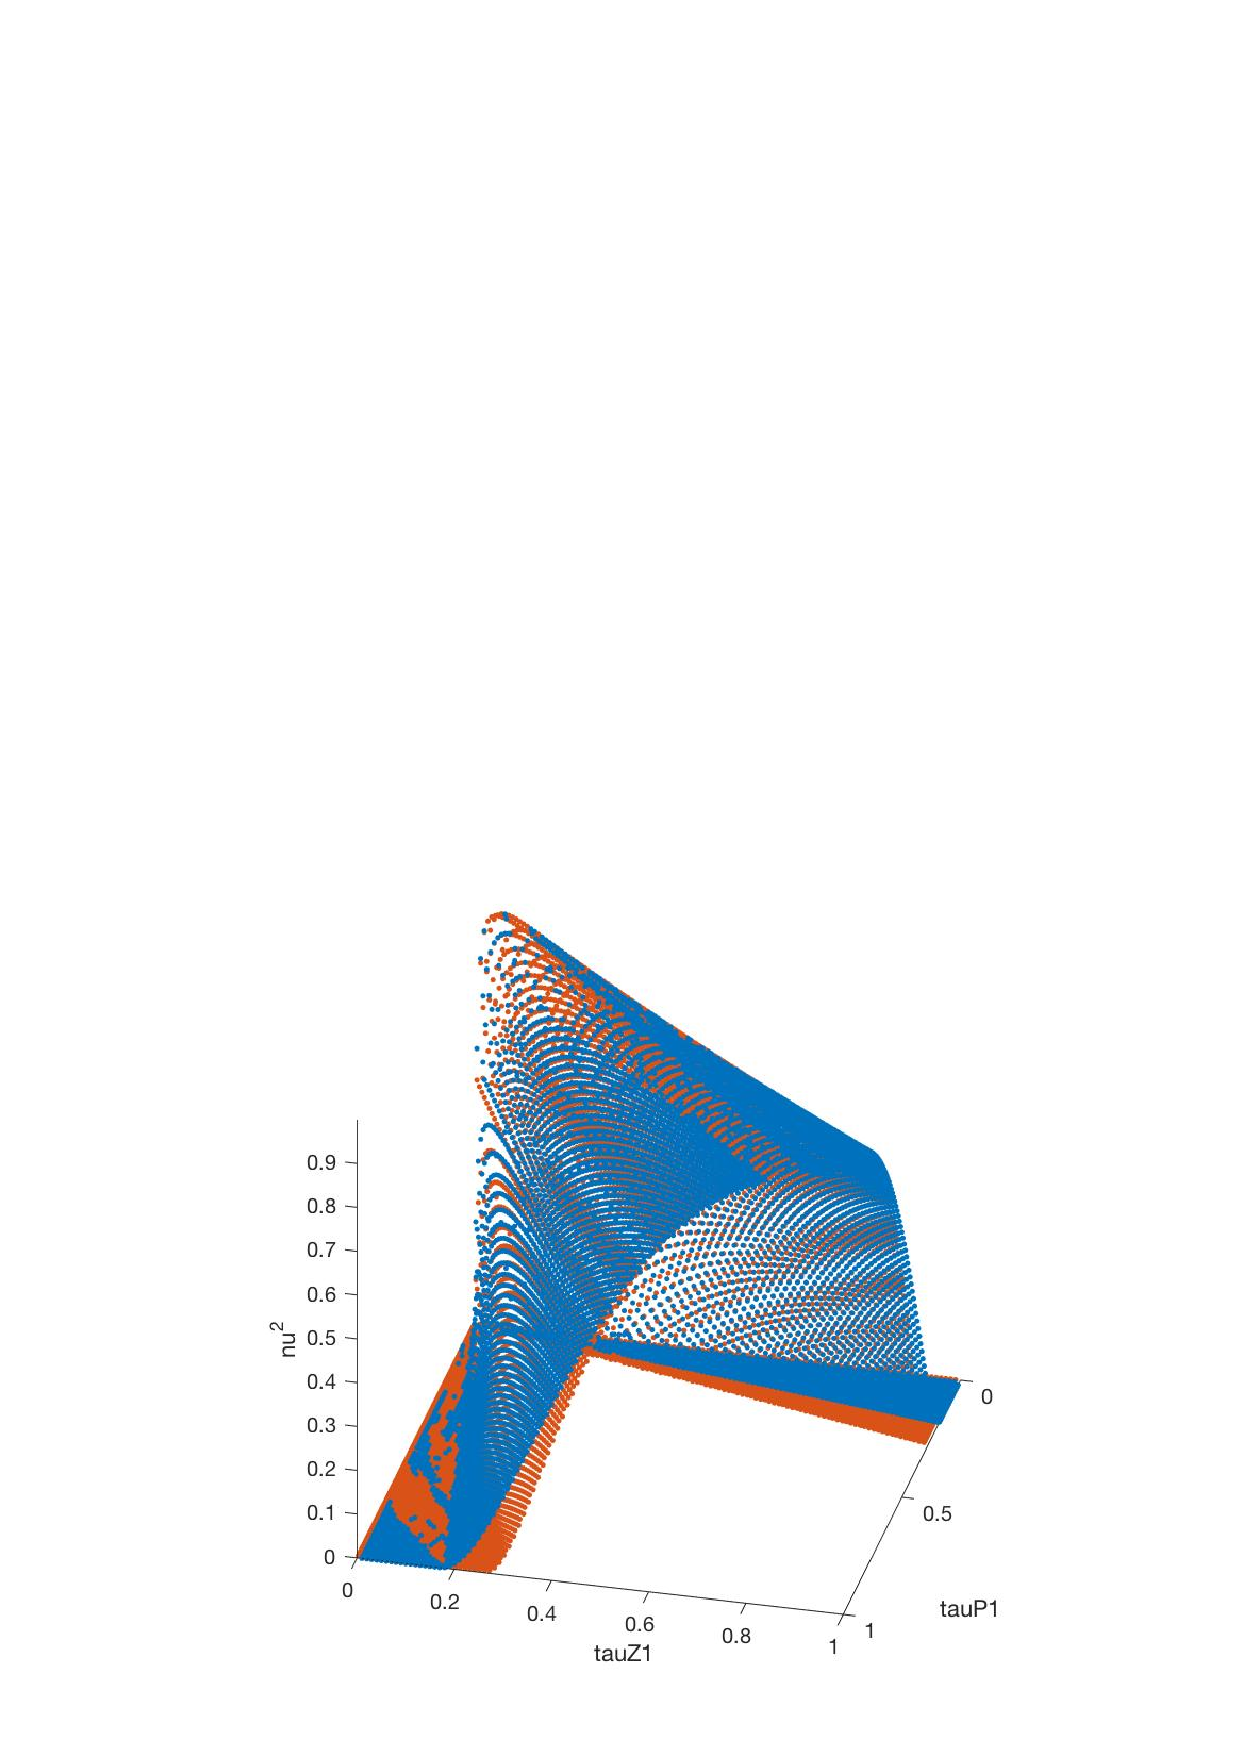
\includegraphics[width=9cm]{images/main.jpg}
\caption{График зависимости $\nu^2$ от $\tau_{p1}, \tau_{p2}$.  Синим цветом представлено точное решение, а оранжевым цветам представлено вычисленное решение параметра $\nu^2$}
\end{figure}

При $B < 0$ уравнение может иметь 2 корня. В этой ситуации потребуем отрицательность дискриминанта:
 \begin{equation}
 \begin{aligned}
&-4\tau_{z1}^4 \varepsilon \delta + 8\tau_{z1}^4 \varepsilon + \tau_{z1}^4 - 16\tau_{z1}^3 \tau_{p1} \varepsilon - 8\tau_{z1}^3 \tau_{p1} + 8\tau_{z1}^2 \tau_{p1}^2 \varepsilon \delta + 8\tau_{z1}^2 \tau_{p1}^2 \varepsilon + 8\tau_{z1}^2 \tau_{p1}^2 \delta + \\
& + 14\tau_{z1}^2 \tau_{p1}^2 - 16\tau_{z1} \tau_{p1}^3 \delta - 8\tau_{z1} \tau_{p1}^3 - 4\tau_{p1}^4 \varepsilon \delta + 8\tau_{p1}^4 \delta + \tau_{p1}^4 \leqslant 0
 \end{aligned}
\end{equation}

 \begin{equation}
 \begin{aligned}
4(\tau_{z1}^2-\tau_{p1}^2)^2(2\varepsilon\tau_{z1}^2-\varepsilon\delta+2\delta\tau_{p1}^2)+(\tau_{z1}-\tau_{p1})^2(\tau_{z1}^2-6\tau_{z1}\tau_{p1}+\tau_{p1}^2)\leqslant 0
 \end{aligned}
\end{equation}

 \begin{equation}
 \begin{aligned}
4(\tau_{z1}+\tau_{p1})^2(2\varepsilon\tau_{z1}^2-\varepsilon\delta+2\delta\tau_{p1}^2)+(\tau_{z1}^2-6\tau_{z1}\tau_{p1}+\tau_{p1}^2)\leqslant 0
 \end{aligned}
\end{equation}

\pagebreak
\subsection{Оценка полосы захвата для систем ФАПЧ с фильтром \\ $\frac{(1+\tau_{z1}x)(1+\tau_{z2}x)}{(1+\tau_{p1}x)(1+\tau_{p2}x)}$}
Оценим полосу захвата для систем ФАПЧ с фильтром, определяемым передаточной функцией:
 \begin{equation}\label{filter3}
 \begin{aligned}
W(s) = \frac{(1+\tau_{z1}s)(1+\tau_{z2}s)}{(1+\tau_{p1}s)(1+\tau_{p2}s)}, \quad 0<\tau_{pi},\tau_{zj} < 1, \quad \tau_{pi} \neq \tau_{zj}, \quad i=1,2, \quad j=1,2
 \end{aligned}
\end{equation}
Введем обозначения:
 \begin{equation}
 \begin{aligned}
\alpha_1 = \tau_{p1} + \tau_{p2}\text{,}\quad 
\alpha_2 = \tau_{p1}\tau_{p2}\text{,}\quad 
\beta_1 = \frac{\tau_{z1}+\tau_{z2}}{\tau_{p1}+\tau_{p2}}\text{,}\quad 
\beta_2 = \frac{\tau_{z1}\tau_{z2}}{\tau_{p1}\tau_{p2}}
 \end{aligned}
\end{equation}
Тогда \eqref{filter3} принимает вид:
 \begin{equation}\label{filter3-1}
 \begin{aligned}
W(s) = \frac{1+\alpha_1\beta_1s + \alpha_2\beta_2s^2}{1+\alpha_1s + \alpha_2s^2}
 \end{aligned}
\end{equation}
Предположим:
 \begin{equation}\label{restriction-1}
 \begin{aligned}
\beta_1 < \beta_2 < 1
 \end{aligned}
\end{equation}
Тогда по теореме ???? пара $(A,B)$ управляема. Заметим
 \begin{equation}
 \begin{aligned}
\text{det}(sI-A) = s^2 + \alpha_1\alpha_2^{-1}s + \alpha_2^{-1}
 \end{aligned}
\end{equation}
Матрица $A$ устойчива. Найдем $\varepsilon, \delta, \varkappa, \tau$ так, что бы максимизировать $\nu$. Для этого подставим \eqref{filter3-1} в \eqref{first_th_eq} и перенесем все в левую часть неравенства. Сделаем замену переменной $t = x^2$. В результате преобразований \eqref{first_th_eq} принимает следующий вид:
 \begin{equation}\label{filter3-th_first-1}
 \begin{aligned}
&\alpha_2^2\tau t^3 + (\alpha_1^2\tau - 2\alpha_2\tau - \alpha_2^2\delta - \alpha_2^2\beta_2^2\varepsilon - \alpha_2^2\beta_2^2\tau + \alpha_2^2\beta_2\varkappa)t^2 +\\
&+ (\tau - \alpha_2\varkappa + 2\alpha_2\delta - \alpha_1^2\delta - \alpha_1^2\beta_1^2\varepsilon - \alpha_1^2\beta_1^2\tau - \alpha_2\beta_2\varkappa + 2\alpha_2\beta_2\varepsilon + 2\alpha_2\beta_2\tau + \alpha_1^2\beta_1\varkappa)t + \\
&+ \varkappa - \varepsilon - \tau - \delta \geqslant 0, \quad \forall t \in \mathbb{R_+}
 \end{aligned}
\end{equation}
Положим $\tau = 0$. И не умаляя общности можем считать $\varkappa = 1$. Тогда \eqref{filter3-th_first-1} принимает вид:
 \begin{equation}\label{filter3-th_first-2}
 \begin{aligned}
&(-\varepsilon\alpha_2^2\beta_2^2 + \alpha_2^2\beta_2 - \delta\alpha_2^2)t^2 + (-\varepsilon\alpha_1^2\beta_1^2 + \alpha_1^2\beta_1 - \delta\alpha_1^2 - \alpha_2 + 2\alpha_2\delta - \alpha_2\beta_2 + 2\alpha_2\beta_2\varepsilon)t +\\
& + 1 - \varepsilon - \delta \geqslant 0, \quad \forall t \in \mathbb{R_+}
 \end{aligned}
\end{equation}
Заметим, что $\varepsilon \leqslant 1 - \delta$ является необходимым условием справедливости \eqref{filter3-th_first-2}. Для максимизации $4\varepsilon\delta$ положим $\varepsilon = 1-\delta$.
 \begin{equation}\label{filter3-3}
 \begin{aligned}
(\alpha_2^2\beta_2 - \alpha_2^2\delta - \alpha_2^2\beta_2^2 + \alpha_2^2\beta_2^2\delta)t + \alpha_2\beta_2 - \alpha_2 + 2\alpha_2\delta + \alpha_1^2\beta_1 - \alpha_1^2\delta - \alpha_1^2\beta_1^2 + \alpha_1^2\beta_1^2\delta - 2\alpha_2\beta_2\delta \geqslant 0
 \end{aligned}
\end{equation}
Так как максимальное значение достигается на границе положим 
 \begin{equation}
 \begin{aligned}
\alpha_2\beta_2 - \alpha_2 + 2\alpha_2\delta + \alpha_1^2\beta_1 - \alpha_1^2\delta - \alpha_1^2\beta_1^2 + \alpha_1^2\beta_1^2\delta - 2\alpha_2\beta_2\delta = 0
 \end{aligned}
\end{equation}
Тогда 
 \begin{equation}\label{filter3_positive_numerator}
 \begin{aligned}
\delta = \frac{\alpha_1^2(1-\beta_1)\beta_1 - \alpha_2(1-\beta_2)}{\alpha_1^2(1-\beta_1^2) - 2\alpha_2(1-\beta_2)}
 \end{aligned}
 \end{equation}
Для того что бы $\delta > 0$ потребуем положительность числителя \eqref{filter3_positive_numerator}, что равносильно
 \begin{equation}
 \begin{aligned}
\alpha_1^2 > \frac{\alpha_2(1-\beta_2)}{\beta_1(1-\beta_1)}
 \end{aligned}
 \end{equation}
Это условие гарантирует положительность знаменателя и $\delta$
 \begin{equation}
 \begin{aligned}
\alpha_1^2(1-\beta_1^2) - 2\alpha_2(1-\beta_2) > \frac{\alpha_2(1-\beta_2)}{\beta_1}(1+\beta_1) - 2\alpha_2(1-\beta_2)= \frac{\alpha_2(1-\beta_2)(1 - \beta_1)}{\beta_1} > 0
 \end{aligned}
 \end{equation}
Получили, что
 \begin{equation}
 \begin{aligned}
\nu^2 < 4\frac{[\alpha_1^2(1-\beta_1) - \alpha_2(1-\beta_2)][\alpha_1^2(1-\beta_1)\beta_1 - \alpha_2(1-\beta_2)]}{[\alpha_1^2(1-\beta_1^2) - 2\alpha_2(1-\beta_2)]^2}
 \end{aligned}
 \end{equation}
 
\pagebreak
\section{Заключение}
В рамках данной работы были рассмотрены три передатоные функции фильтра: 
 \begin{align}
&W(s) = \frac{1}{(1+\tau_{p1}s)(1+\tau_{p2}s)}\label{first}\\[5pt]
&W(s) = \frac{(1+\tau_{z1}s)^2}{(1+\tau_{p1}s)^2}\label{second}\\[5pt]
&W(s) = \frac{(1+\tau_{z1}x)(1+\tau_{z2}x)}{(1+\tau_{p1}x)(1+\tau_{p2}x)}\label{third}
 \end{align}
 Для \eqref{first}, \eqref{second} были получены аналитические оценки полосы захвата, которые были подтверждены численно. Полоса захвата систем ФАПЧ с фильтром, определяемым передаточной функцией \eqref{third} исследовалась ранее Леоновым~Г.\:А. Для нее был восстановлен вывод. 
 
 В настоящее время системы фазовой автоподстройки частоты используются в различных устройствах. Аналитические оценки, полученные в данной работе, могут быть интерсны инженерам и могут использоваться при проектировании и реализации систем ФАПЧ 3 порядка.
\pagebreak
\begin{thebibliography}{3}
\bibitem{UsageOfThirdOrder1}
Ms. Ujwala A. Belorkar  and Dr. S.A.Ladhake ,Dssign of loe power phase Locked Loop (PLL) using 45NM VLSI  TECHNOLOGY,International  journal of  VLSI  design  \&  Communication  Systems (  LSICS  ), Vol.1, No.2, June 2010
\bibitem{UsageOfThirdOrder2}
Gursharan Reehal, A Digital Frequency Synthesizer Using Phase Locked Loop Technique” 1998
\bibitem{Microprocessors}
 KengL.WongIanA.Young,JeffreyK.Greason. Apllclockgenerator with 5 to 110 mhz of lock range for microprocessors. IEEE Journal of Solid-State Circuits, 27, 1992. 
 \bibitem{thirdOrderPLL}
 Lin Feng, Chu Wu, Bo Jin, Zhen Yu Wu. A Passive Third-Order Cascade PLL Filter
 \bibitem{best}  Best~R.\:E. Phase-Locked Loops: Design, Simulation, and Applications / New York: McGraw-Hill Education, 2007. P.~115--116.
\bibitem{kuznetsov}  Leonov~G.\:A., Kuznetsov~N.\:V. Nonlinear mathematical models of phase-locked loops : stability and oscillations / Cambridge: Cambridge Scientific Publishers, 2014. P.~112--113.
\bibitem{leonov}  Leonov~G.\:A., Reitmann~V., Smirnova~V.\:B. Non-Local Methods for Pendulum-Like Feedback Systems / ed. by H.~Kurke. Wiesbaden: Vieweg+Teubner Verlag, 1992. P.~72--75.
\bibitem{kuznetsov_article} Kuznetsov~N.\:V., Leonov~G.\:A., Yuldashev~M.\:V., Yuldashev~R.\:V. Hold-In, Pull-In, and Lock-In Ranges of PLL Circuits: Rigorous Mathematical Definitions and Limitations of Classical Theory // Transactions on Circuits and Systems I: Regular Papers. 2015. Vol.~62, No~10. P.~2455.
\bibitem{thirdOrderPLL} Feng~L., Wu~C., Jin~B., Wu~Z. A Passive Third-order Cascade PLL Filter // Trans Tech Publications. 2011. Vol. 255-260. P.~2262.
\bibitem{shahgildyan}  Шахгильдян~В.\:В., Ляховкин~А.\:А. Системы фазовой автоподстройки частоты / М.:~Изд-во Связь, 1972. P.~15--19.
\bibitem{rao}  Rao~R.\:B., Kunysz~W., Fante~R., McDonald~K., GPS/GNSS Antennas / Boston: Artech House, 2013. P.~50--51.
\end{thebibliography}
\end{document}  
% КОНЕЦ ДОКУМЕНТА !